\begin{frame}[fragile]{Tutorial: Two-site states}

\begin{columns}

\begin{column}{5cm}

\begin{onlyenv}<1->
\begin{lstlisting}[language=JuliaLocal, style=julia, basicstyle=\small]
ψ = ITensor(i1, i2)
ψ[i1=>1, i2=>2] = 1/√2
ψ[i1=>2, i2=>1] = 1/√2

ψ = (Zp1 * Zm2 +
        Zm1 * Zp2)/√2
\end{lstlisting}
\end{onlyenv}

\begin{onlyenv}<3->
\begin{lstlisting}[language=JuliaLocal, style=julia, basicstyle=\small]
inner(ψ, ψ)
inner(ZpZm, ψ)

U, S, V = svd(ZmZp, i1)
s = diag(S)

U, S, V = svd(ψ, i1)
s = diag(S)
\end{lstlisting}
\end{onlyenv}

\end{column}

\begin{column}{5cm}

\begin{onlyenv}<1-1>
(|Z+$\rangle$|Z-$\rangle$ + |Z-$\rangle$|Z+$\rangle$)/√2 \\
~\\
~\\
~\\
From single-site states \\
\end{onlyenv}

\begin{onlyenv}<2->
\vspace*{0.0cm}
\begin{center}
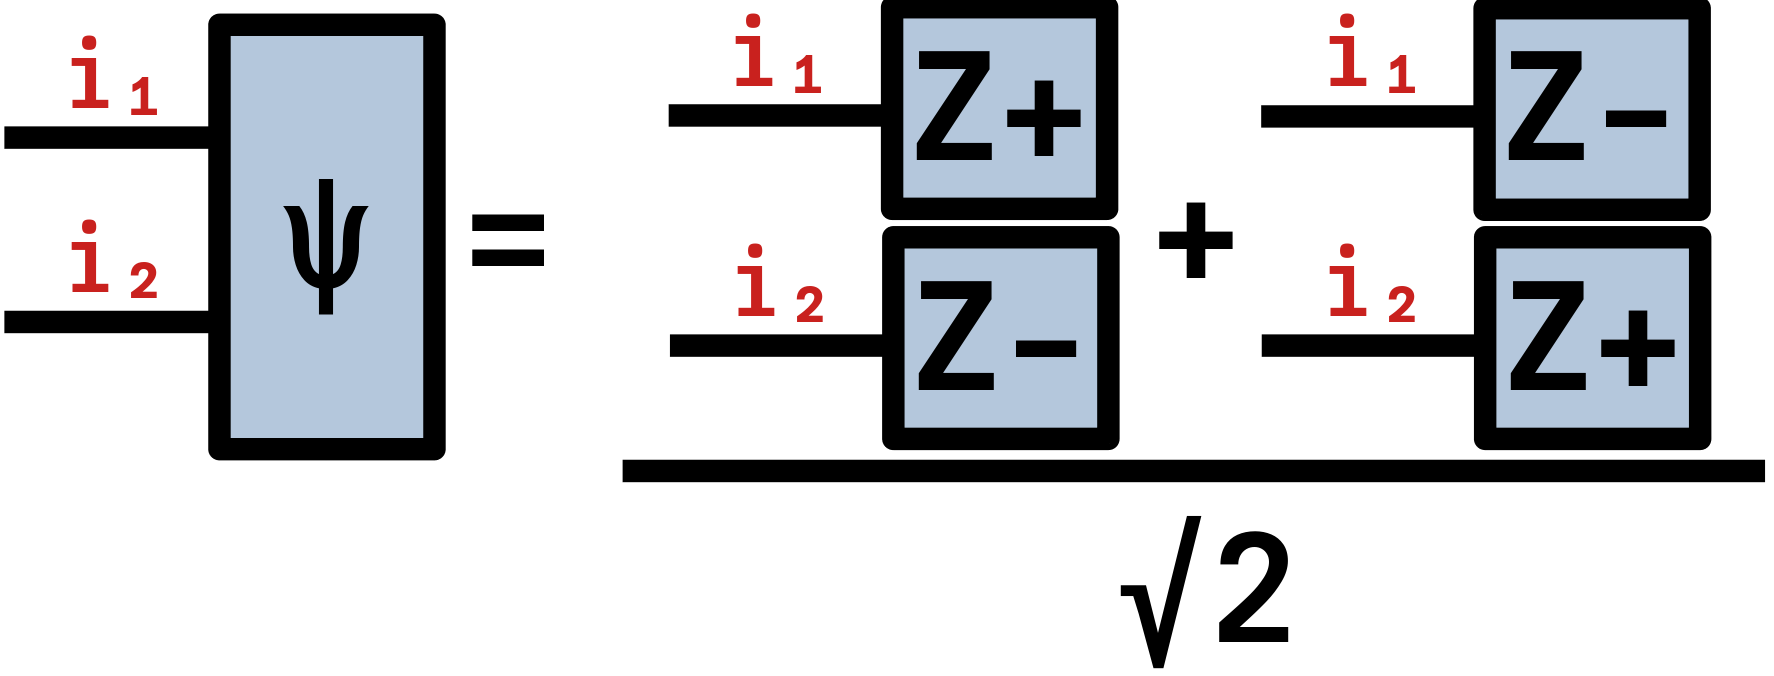
\includegraphics[width=0.2\textwidth]{
  slides/assets/cat12.png
}
\end{center}
\vspace*{0.0cm}
\end{onlyenv}

\begin{onlyenv}<3-3>
$\approx$ 1 \\
$\approx$ 1/√2 \\
~\\
~\\
$\approx$ [1, 0] \\
~\\
~\\
$\approx$ [1/√2, 1/√2]
\end{onlyenv}

\begin{onlyenv}<4->
\vspace*{0.0cm}
\begin{center}
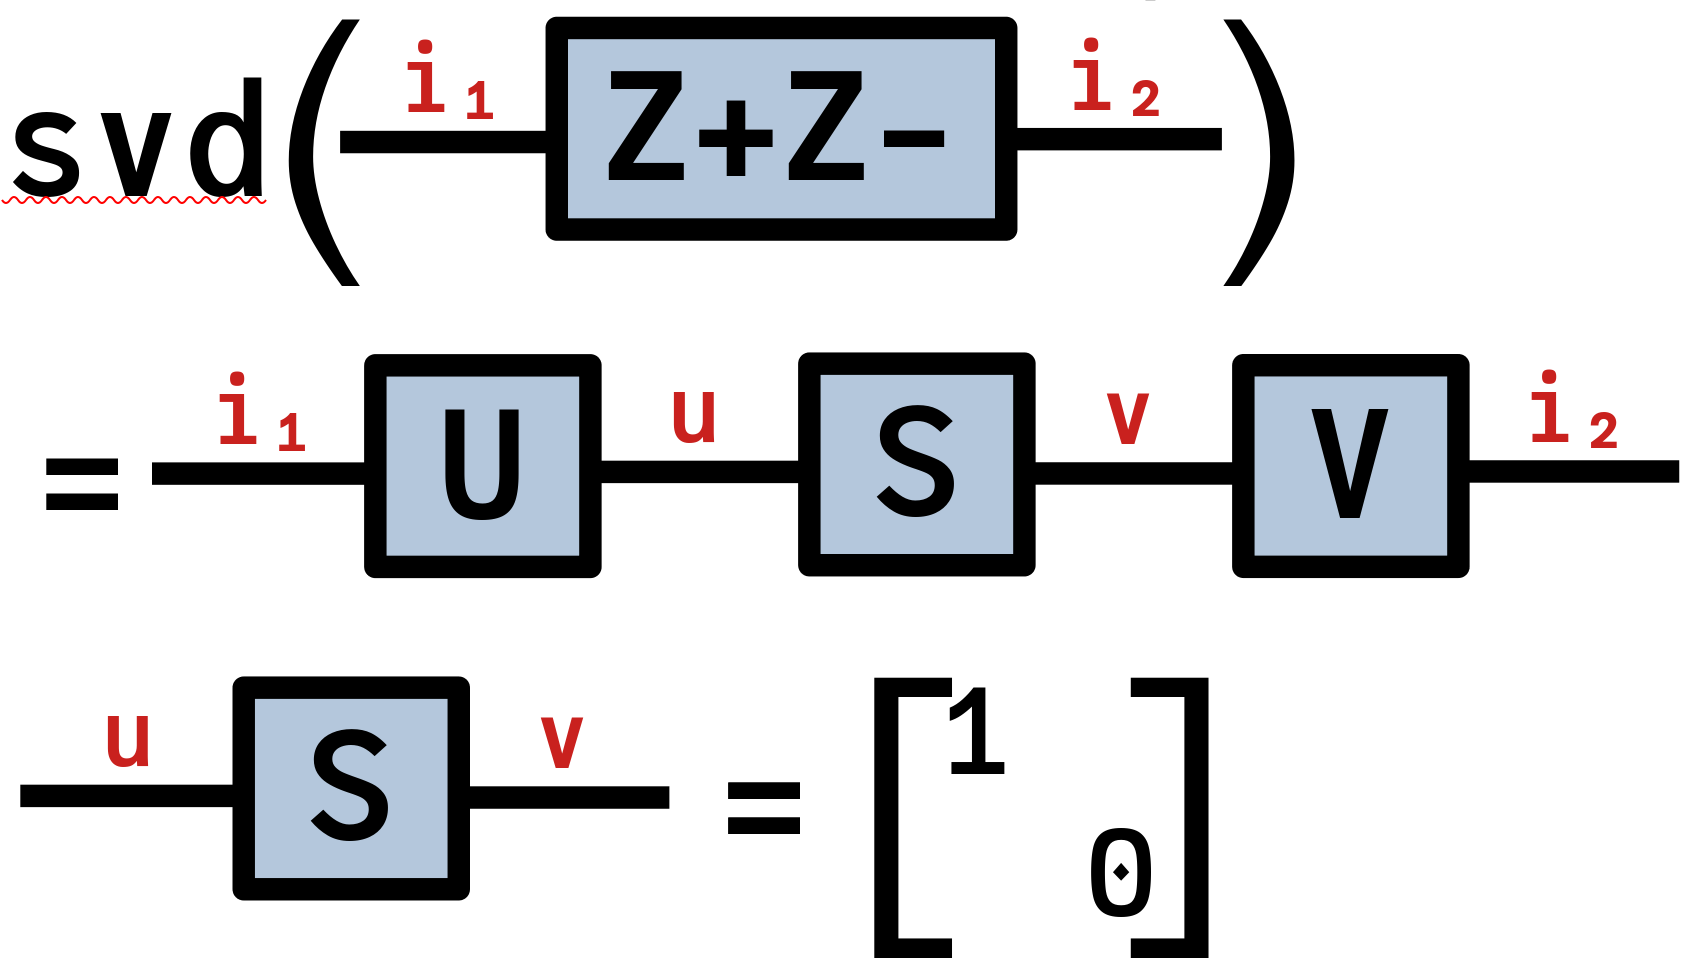
\includegraphics[width=0.2\textwidth]{
  slides/assets/svd_ZpZm12.png
} \\
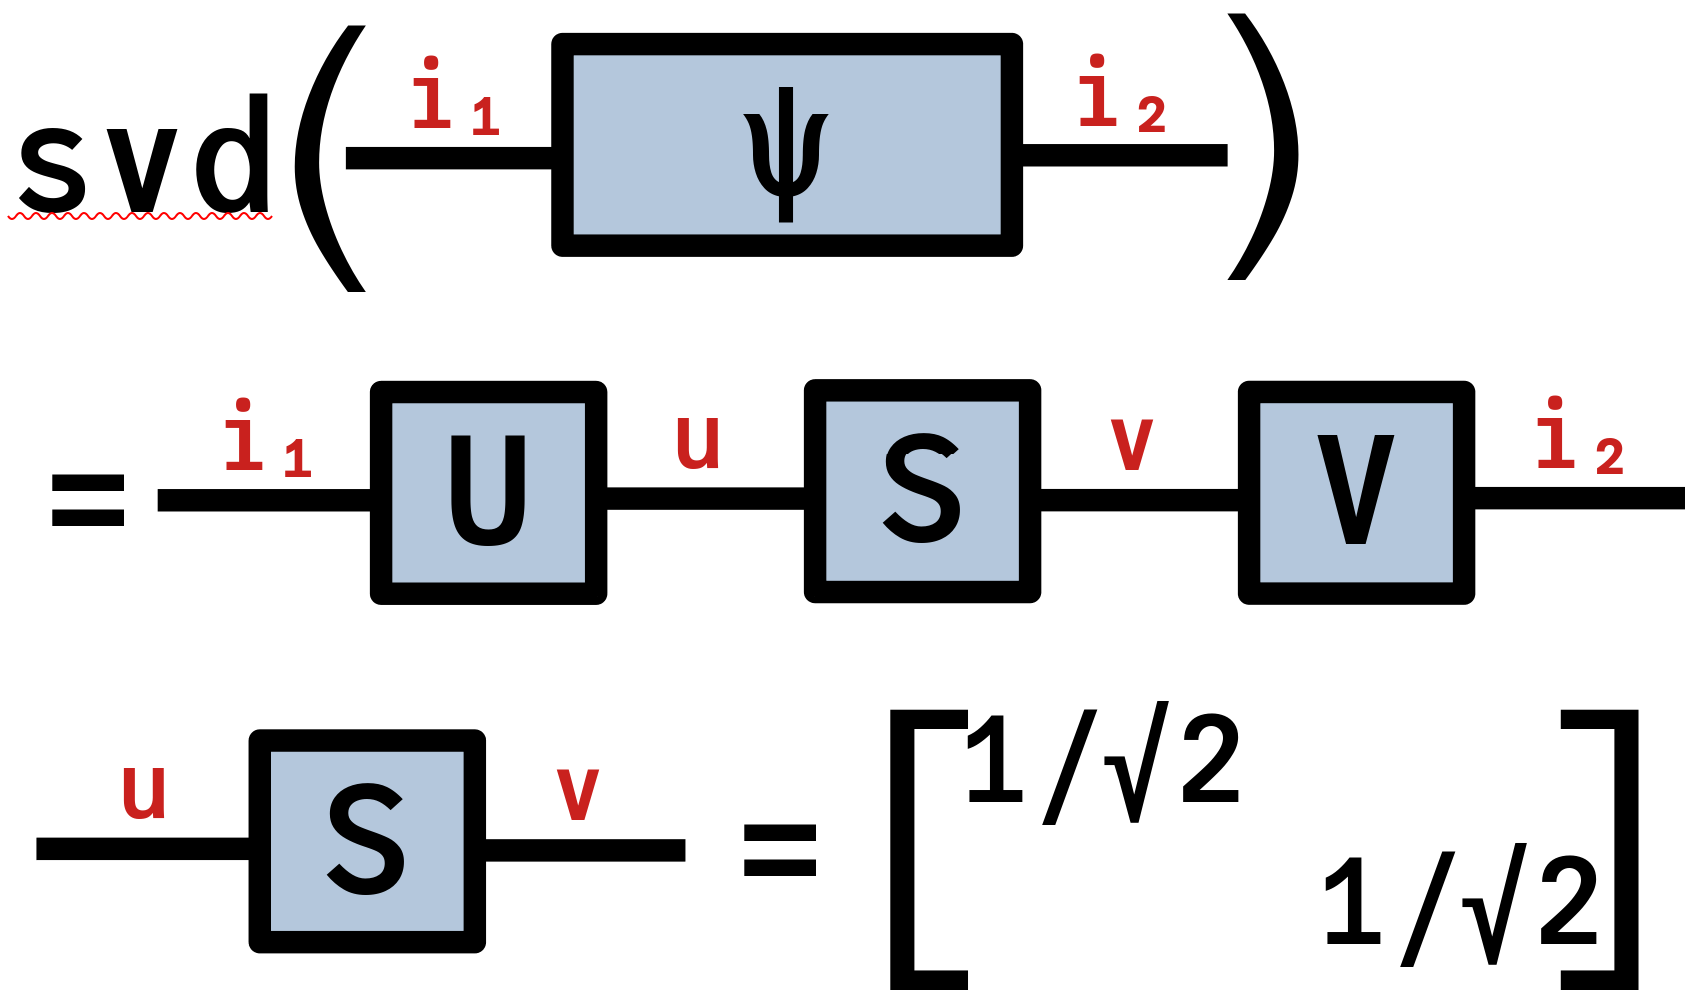
\includegraphics[width=0.2\textwidth]{
  slides/assets/svd_cat12.png
}
\end{center}
\vspace*{0.0cm}
\end{onlyenv}

\end{column}

\end{columns}

\end{frame}
